\documentclass[a4paper,12pt]{article}
\usepackage[utf8]{inputenc}
\usepackage{xcolor}
\usepackage{graphicx}
\usepackage{geometry}
\usepackage{background}
\backgroundsetup{contents={}} % Esto debería limpiar cualquier contenido predeterminado

\usepackage{eso-pic}
\usepackage{fancyhdr}
\usepackage{tikz}

\geometry{top=2cm, bottom=2.54cm, left=2.2cm, right=2.54cm}

% Definir el color usando un código hexadecimal
\definecolor{Penta}{HTML}{220d47}

% Configuración del fondo de la portada
\newcommand\BackgroundPic{
    \AddToShipoutPicture*{
        \begin{tikzpicture}[remember picture, overlay]
            % Fondo de color Penta
            \fill[Penta] (current page.north west) rectangle (current page.south east);
        \end{tikzpicture}
    }
}

\newcommand\OverlayPentagon{
    \AddToShipoutPicture*{
        
\begin{tikzpicture}[remember picture, overlay, scale=10, opacity=0.2]
            % Pentágono superpuesto
            \draw[line width=4pt, Penta] (current page.center) ++(-0.5,-0.5) -- ++(1,0) -- ++(0.309,0.951) -- ++(-0.809,0.587) -- ++(-1.309,-0.951) -- cycle;
        \end{tikzpicture}
    }
}

% Ajustar headheight según la advertencia
\setlength{\headheight}{30pt}

% Configuración del encabezado y pie de página
\fancypagestyle{mystyle}{
    \fancyhf{}
    \fancyhead[L]{
            \makebox[0pt][l]{
            \hspace{-1cm}\includegraphics[width=0.16\textwidth]{images/header.png}}
    }
    \fancyfoot[R]{
        \raisebox{0pt}{\makebox[0pt][l]{
            \hspace{0.2cm}
        \begin{tikzpicture}[baseline=(current bounding box.center)]
            \draw[draw=Penta, line width=2pt] (0,0) -- (1,0) -- (1.309,0.951) -- (0.5,1.538) -- (-0.309,0.951) -- cycle;
            \node at (0.5,0.75) {\thepage};
        \end{tikzpicture}
        }}
    }
    \renewcommand{\headrulewidth}{0pt}
    \renewcommand{\footrulewidth}{0pt}
}

\begin{document}

% Generar la portada
\BackgroundPic
\OverlayPentagon
\begingroup
\thispagestyle{empty} % Sin número de página ni encabezado en la primera página
\color{white}
\centering
\vspace*{\fill}
{\Huge\bfseries contenido-titulo}
\vspace*{\fill}
\clearpage
\endgroup

% Aplicar estilo para el resto de las páginas
\pagestyle{mystyle}

% Configuración del fondo de las páginas internas
\backgroundsetup{
  scale=16,
  color=black,
  opacity=0.2,
  angle=0,
  position=current page.south west,
  vshift=20pt,
  hshift=10pt,
  contents={%
        
\begin{tikzpicture}
            \fill[Penta] (0,0) -- (1,0) -- (1.309,0.951) -- (0.5,1.538) -- (-0.309,0.951) -- cycle;
        \end{tikzpicture}
  }
}

% Inclusion de contenido
\include{src/contenido-reemplazable }

\end{document}
